%Shortest path problem
\section{Shortest path problem}\label{shortestPathProblem}
	For route planning, routes through a network must be optimized in regards to one or even many criteria.
	A common criteria is the \textit{travel time}. Others include cost, number of transfers or restrictions
	in transportation types.
	
	In this chapter, we will first give an informal description of the \earliestArrivalProblem. Followed by
	the \shortestPathProblem, which is equivalent to the \earliestArrivalProblem for our graph-based network
	representations.
	
	Then, we introduce algorithms for solving the problem. First, for time-independent networks, then for time-dependent.
	Afterwards, we explain two solutions for combined networks, using multiple transportation modes. There, the problem
	description slightly changes by adding transportation mode restrictions.\\\\
	\begin{mydef}
		The earliest arrival problem asks for finding a \textnormal{route} in a network with following properties
		\begin{itemize}
			\item[1.] The route must start at $s$ and end at $t$.
			\item[2.] The departure time at $s$ is $\tau$.
			\item[3.] All other applicable routes must have a greater travel time, i.e. arrive later at $t$.
		\end{itemize}
		Points $s$ and $t$ are given source and target points in the network respectively. $\tau$ is the desired departure time,
		it may be ignored for a time-independent network.
	\end{mydef}
	\begin{mydef}
		Given a graph $G = (V, E)$, source and target nodes $s, t \in V$ and a desired departure time $\tau$, the shortest path
		problem asks for a path $p$ (see \defref{path}) which
		\begin{itemize}
			\item[1.] begins at $s$ and ends at $t$,
			\item[2.] has the smallest weight of all applicable paths.
		\end{itemize}
		The arrival time at $t$ is $\tau$ plus the weight of $p$. In a time-dependent
		graph $\tau$ must be used to ensure correct edge weights. The path $p$ is called \textnormal{shortest path}.
	\end{mydef}\quad\\
	Additionally, we consider a special variant of the shortest path problem:
	\begin{mydef}
		The many-to-one shortest path problem is a variation of the shortest path problem
		where the source consists of a set of source nodes $S \subseteq V$.

		The problem asks for the path $p$ that starts at the source $s \in S$ which minimizes the path weight.
	\end{mydef}

%Time-independent
\subsection{Time-independent}
	Route planning in time-independent networks is a very well studied problem.
	Many efficient solutions to the shortest path problem exists. We introduce a very basic algorithm, \dijkstra
	and a simple improvement based on heuristics, \astar.
	% Time-independent example
	\begin{figure}[!ht]
		 \begin{center}
			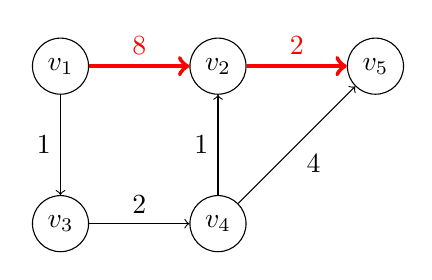
\begin{tikzpicture}[y = -1cm]
			 	% Nodes
			 	\node[circle, draw] (v1) at (0, 0) {$v_1$};
			 	\node[circle, draw] (v2) at (2, 0) {$v_2$};
			 	\node[circle, draw] (v3) at (0, 2) {$v_3$};
			 	\node[circle, draw] (v4) at (2, 2) {$v_4$};
			 	\node[circle, draw] (v5) at (4, 0) {$v_5$};
			 	
			 	% Edges
			 	\draw[ultra thick, ->, color = red] (v1) to node[above] {$8$} (v2);
			 	\draw[ultra thick, ->, color = red] (v2) to node[above] {$2$} (v5);
			 	\draw[->] (v1) to node[left] {$1$} (v3);
			 	\draw[->] (v3) to node[above] {$2$} (v4);
			 	\draw[->] (v4) to node[left] {$1$} (v2);
			 	\draw[->] (v4) to node[below right] {$4$} (v5);
			\end{tikzpicture}\qquad\qquad\qquad
			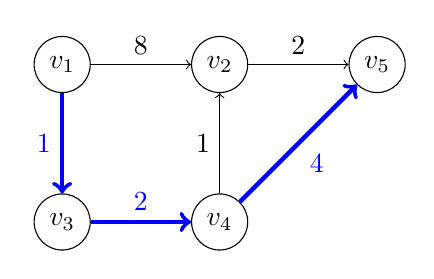
\begin{tikzpicture}[y = -1cm]
			 	% Nodes
			 	\node[circle, draw] (v1) at (0, 0) {$v_1$};
			 	\node[circle, draw] (v2) at (2, 0) {$v_2$};
			 	\node[circle, draw] (v3) at (0, 2) {$v_3$};
			 	\node[circle, draw] (v4) at (2, 2) {$v_4$};
			 	\node[circle, draw] (v5) at (4, 0) {$v_5$};
			 	
			 	% Edges
			 	\draw[->] (v1) to node[above] {$8$} (v2);
			 	\draw[->] (v2) to node[above] {$2$} (v5);
			 	\draw[ultra thick, ->, color = blue] (v1) to node[left] {$1$} (v3);
			 	\draw[ultra thick, ->, color = blue] (v3) to node[above] {$2$} (v4);
			 	\draw[->] (v4) to node[left] {$1$} (v2);
			 	\draw[ultra thick, ->, color = blue] (v4) to node[below right] {$4$} (v5);
			\end{tikzpicture}\quad\\\phantom{v}\quad\\
			\begin{tikzpicture}[y = -1cm]
			 	% Nodes
			 	\node[circle, draw] (v1) at (0, 0) {$v_1$};
			 	\node[circle, draw] (v2) at (2, 0) {$v_2$};
			 	\node[circle, draw] (v3) at (0, 2) {$v_3$};
			 	\node[circle, draw] (v4) at (2, 2) {$v_4$};
			 	\node[circle, draw] (v5) at (4, 0) {$v_5$};
			 	
			 	% Edges
			 	\draw[->] (v1) to node[above] {$8$} (v2);
			 	\draw[ultra thick, ->, color = darkgreen] (v2) to node[above] {$2$} (v5);
			 	\draw[ultra thick, ->, color = darkgreen] (v1) to node[left] {$1$} (v3);
			 	\draw[ultra thick, ->, color = darkgreen] (v3) to node[above] {$2$} (v4);
			 	\draw[ultra thick, ->, color = darkgreen] (v4) to node[left] {$1$} (v2);
			 	\draw[->] (v4) to node[below right] {$4$} (v5);
			\end{tikzpicture}
		\end{center}
		\caption{Example for a time independent network, represented by a road graph.
		The figure shows three paths from $v_1$ to $v_5$. From top left to bottom right, the path
		weights are $10$, $7$ and $6$. The last example represents the shortest path from $v_1$ to $v_5$.}
		\label{timeIndependentExample}
	\end{figure}\quad\\
	The network shown by \figref{timeIndependentExample} acts as toy example for this section.

%Dijkstra
\subsubsection{Dijkstra}
	\dijkstra \libref{dijkstra} is a simple approach to solving the shortest path problem. It can be viewed
	as the logical extension of breadth-first search (\bfs) \libref{dijkstra} in weighted graphs. The algorithm
	revolves around a priority queue where it stores neighboring nodes, sorted by their shortest path cost.
	In each round, the node with the smallest shortest path cost is \textit{relaxed}. That is, all its neighboring,
	not already relaxed, nodes are added to the queue. The algorithm terminates as soon as the target node has been relaxed.
	\algoref{dijkstra} gives a formal description.
	% Dijkstra implementation
	\IncMargin{1em}
	\begin{algorithm}
		\SetKwInOut{Input}{input}
  		\SetKwInOut{Output}{output}
  		\SetKw{Break}{break}
  		\SetKwData{undef}{undefined}\SetKwData{currentDist}{currentDist}
		\SetKwFunction{dist}{dist}\SetKwFunction{prev}{prev}
		\BlankLine
		\Input{graph $G = (V, E)$, source $s \in V$, target $t \in V$}
		\Output{shortest path from $s$ to $t$}
		\BlankLine
		\tcp{Initialization}
		\For{$v \in V$}{
			$\dist(v) \leftarrow \infty$\;
			$\prev(v) \leftarrow \undef$\;
		}
		\BlankLine
		$\dist(s) \leftarrow 0$\;
		$Q \leftarrow \{s\}$\;
		\BlankLine
		\tcp{Compute shortest paths}
		\While{$Q$ is not empty}{
			$u \leftarrow \argmin_{u' \in Q} \dist(u')$\;
			$Q \leftarrow Q \setminus \{u\}$\;
			\BlankLine
			\If{$u == t$}{
				\Break\;
			}
			\BlankLine
			\tcp{Relax $u$}
			\For{outgoing edge $(u, w, v) \in E$}{
				$\currentDist \leftarrow \dist(u) + w$\;
				\If{$\currentDist < \dist(v)$}{
					\tcp{Improve distance by using this edge}
					$\dist(v) \leftarrow \currentDist$\;
					$\prev(v) \leftarrow u$\;
					$Q \leftarrow Q \cup \{v\}$\;
				}
			}
		}
		\BlankLine
		\tcp{Extract path by backtracking}
		$p \leftarrow$ empty path\;
		$u \leftarrow t$\;
		\While{$\prev(u) \neq \undef$}{
			$w \leftarrow \dist(u) - \dist(\prev(u))$\;
			prepend $(\prev(u), w, u)$ to $p$\;
			$u \leftarrow \prev(u)$\;
		}
		prepend $s$ to $p$\;
		\Return $p$\;
		\BlankLine
		\caption{Dijkstra's algorithm for computing shortest paths in time-independent graphs.}\label{dijkstra}
	\end{algorithm}\DecMargin{1em}\quad\\\\
	To familiarize with the algorithm, we step through the execution for the graph shown by \figref{timeIndependentExample},
	with $v_1$ as source and $v_5$ as target node.
	
	The $\dist$ function, often implemented as array, stores the tentative shortest path weight to the given node.
	$\prev$ is used for path extraction at the end, it stores the parent nodes used for the shortest paths represented by $\dist$.
	The algorithm starts by initializing both collections with default values. Initially the distance to all nodes, except the source, is unknown.
	Thus, $\infty$ is used for them. $Q$ represents the list of nodes that need to be processed, usually implemented as priority queue.
	Initially, it only holds the source node $s$.
	
	In the example $Q$ is initially $\{v_1\}$. The algorithm then relaxes $v_1$ and stores distances to its neighbors:
	\begin{center}
		\begin{tabular}{CC}
			\dist(v_2) = 8	&\prev(v_2) = v_1,\\
			\dist(v_3) = 1	&\prev(v_3) = v_1
		\end{tabular}
	\end{center}
	Additionally, the queue $Q$ is updated, it is
	\begin{align*}
		Q	&= \{v_2, v_3\}.
	\end{align*}
	The next iteration of the loop starts and the node with the smallest distance is chosen, i.e. $v_3$. The node is relaxed and we receive
	\begin{center}
		\begin{tabular}{CC}
			\dist(v_4) = 3	&\prev(v_4) = v_3,\\
			\multicolumn{2}{c}{$Q = \{v_2, v_4\}.$}
		\end{tabular}
	\end{center}
	The next node is $v_4$, yielding
	\begin{center}
		\begin{tabular}{CC}
			\dist(v_2) = 4	&\prev(v_2) = v_4,\\
			\dist(v_5) = 7	&\prev(v_5) = v_4,\\
			\multicolumn{2}{c}{$Q = \{v_2, v_5\}.$}
		\end{tabular}
	\end{center}
	Note that $v_4$ improves the distance to $v_2$. The previous values for $v_2$ are overwritten and the
	tentative shortest path to $v_2$ uses $(v_4, 1, v_2)$ and not $(v_1, 8, v_2)$ anymore.
	In the next round $v_2$ is relaxed which improves the distance to $v_5$:
	\begin{center}
		\begin{tabular}{CC}
			\dist(v_5) = 6	&\prev(v_5) = v_2,\\
			\multicolumn{2}{c}{$Q = \{v_5\}.$}
		\end{tabular}
	\end{center}
	The only node left is the target node $v_5$ now. It is relaxed and the loop terminates.
	The algorithm backtracks the parent pointer
	\begin{align*}
		\prev(v_5)	&= v_2,\\
		\prev(v_2)	&= v_4,\\
		\prev(v_4)	&= v_3,\\
		\prev(v_3)	&= v_1,\\
		\prev(v_1)	&= \vundef
	\end{align*}
	and constructs the shortest path
	\begin{align*}
		p	&= (v_1, 1, v_3)(v_3, 2, v_4)(v_4, 1, v_2)(v_2, 2, v_5)
	\end{align*}
	which is the path shown by the last example in the figure.

%A*
\subsubsection{\astar and \alt}\label{alt}
	An important observation of \dijkstra is that, if it settles the shortest path distance to a node, then,
	all nodes which are closer to the source, were already settled in a previous round.
	
	Moreover, the algorithm explores the graph in all directions equally. It has no sense of \textit{goal direction}.\\\\
	The \astar algorithm \libref{alt} is a simple extension of \dijkstra which improves its efficiency by steering the
	exploration more towards the target. \figref{dijkstra_vs_astar} illustrates this by comparing the \textit{search space}
	of both algorithms. The search space of \astar is smaller and much more directed to the target node $t$.
	% A-star vs Dijkstra
	\begin{figure}[!ht]
		 \begin{center}
			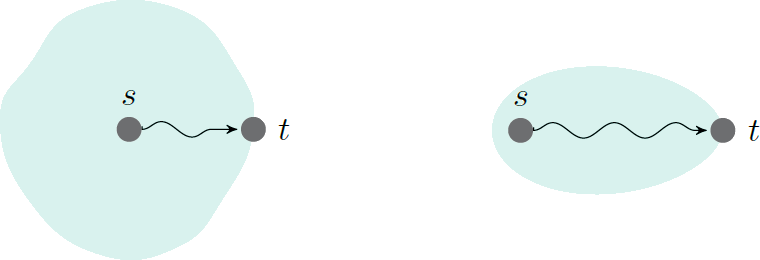
\includegraphics[scale=0.5]{res/dijkstra_vs_astar}
		\end{center}
		\caption{Schematic illustration of a query processed by \dijkstra (left) and \astar (right).
			The highlighted areas indicate the \textit{search space}, i.e. the nodes the algorithm has explored already.
			The illustration is from \libref{routePlanningOverview}.}
		\label{dijkstra_vs_astar}
	\end{figure}\quad\\
	Unfortunately, computing the exact goal direction is equivalent to computing the shortest path to the target.
	Therefore, a heuristic is used to approximate the direction. The choice of the heuristic heavily depends on the underlying network.
	In the worst case, a heuristic may not improve over \dijkstra and the same search space is received. In the best case,
	the algorithm explores only the nodes on the shortest path.
	
	Such a heuristic must fulfill two properties, formulated by \defref{heuristic}.
	\begin{mydef}\label{heuristic}
		Given a graph $G = (V, E)$, a metric $\dist$ on the set $V$ (see \defref{metric}), a \textnormal{heuristic} $h$
		is a metric on $V$ which approximates $\dist$. The heurstic $h$ must be
		\begin{itemize}
			\item[1.] \textnormal{admissable}, i.e. never overestimate:
				\begin{align*}
					\forall u, t \in V: h(u, t) \le \dist(u, t)
				\end{align*}
			\item[2.] \textnormal{monotone}, i.e. satisfy the triangle inequality:
				\begin{align*}
					\forall t \in V\,\forall (u, w, v) \in E: h(u, t) \le w + h(v, t)
				\end{align*}
		\end{itemize}
	\end{mydef}
	\todo{Write something...}

%Time-dependend
\subsection{Time-dependend}
	Blabla

%Connection scan
\subsubsection{Connection scan}\label{csa}
	Blabla

%Multi-modal
\subsection{Multi-modal}
	Blabla

%Modified Dijkstra
\subsubsection{Modified Dijkstra}\label{modifiedDijkstra}
	Blabla

%Access nodes
\subsubsection{Access nodes}\label{accessNodes}
	Blabla

%Other algorithms
\subsection{Other algorithms}
	Blabla